%!TEX root = main.tex

\section{Newton-Raphson's Method}

\subsection{Newton-Raphson Method to search for roots of univariate functions}

In order to find a good estimation of $\sqrt{2}$ with many decimal places, we allow a computer to find better and better approximations of the root  of the polynomial $p(x)=x^2-2$.  We start with an initial guess, say $x_0=3$.  We construct a sequence $\{ x_n \}_{n\in\field{N}}$ that converges to $\sqrt{2}$ as follows:
\begin{enumerate}
\item Find the tangent line to the graph of $p$ at $x_0$, 
\begin{equation*}
y-p(x_0)=p'(x_0)(x-x_0)
\end{equation*}
\item Provided this line is not horizontal ($p'(x_0)\neq 0$), report the intersection of this line with the $x$--axis.  Call this intersection $x_1$
\begin{equation*}
x_1=x_0-\frac{p(x_0)}{p'(x_0)}
\end{equation*}
\item Repeat this process, to get the sequence 
\begin{equation*}
x_{n+1} = x_n - \frac{p(x_n)}{p'(x_n)} = x_n - \frac{x_n^2-2}{2x_n}=\frac{x_n}{2}-\frac{1}{x_n}.
\end{equation*}
\end{enumerate}
\begin{figure}[ht!]
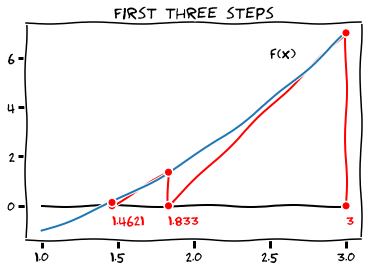
\includegraphics[width=0.6\linewidth]{images/newton1.png}
\caption{Newton-Raphson iterative method}
\label{figure:Newton-Raphson}
\end{figure}
Note the result of applying this process a few times:
\begin{center}
% \begin{table}[ht!]
\begin{tabular}{|c|c|r|} \hline 
$n$ & $x_n$ & $p(x_n)$ \\ \hline \hline 
$0$ & $3.000000000000000$ & $7.0000E+00$ \\ \hline 
$1$ & $1.833333333333333$ & $1.3611E+00$ \\ \hline 
$2$ & $1.462121212121212$ & $1.3780E-01$ \\ \hline 
$3$ & $1.414998429894803$ & $2.2206E-03$ \\ \hline 
$4$ & $1.414213780047198$ & $6.1568E-07$ \\ \hline 
$5$ & $1.414213562373112$ & $4.7518E-14$ \\ \hline 
$6$ & $1.414213562373095$ & $-4.4409E-16$ \\ \hline 
$7$ & $1.414213562373095$ & $4.4409E-16$ \\ \hline 
\end{tabular}
% \caption{Newton-Raphson method: Convergence to $\sqrt{2}$ with 15-digit accuracy in 6 steps}
% \label{table:Newton-Raphson}
% \end{table}
\end{center}

\begin{definition}\index{Newton-Raphson!iteration}\index{Newton-Raphson!method}\index{Newton-Raphson!}\index{Newton-Raphson!recursive formula}
Given a differentiable real-valued function $f\colon \field{R} \to \field{R}$ and an initial guess $x_0 \in \field{R}$, we define the \emph{Newton-Raphson iteration} to be the sequence given by the following \emph{recursive formula}
\begin{equation*}
x_{n+1} = x_n - \frac{f(x_n)}{f'(x_n)}
\end{equation*}
The \emph{Newton-Raphson method} refers to employing this sequence to search and approximate roots of the equation $f(x) = 0$.
\end{definition}

\begin{example}\label{example:NewtonRaphsonChoice}
Consider now the function $f(x) = 1-\tfrac{1}{x}$ over $(0, \infty)$, which has the obvious root $x=1$. The Newton-Raphson method gives the following iterates for any $x_0 \in (0,\infty)$:
\begin{align*}
x_{n+1} = x_n - \frac{f(x_n)}{f'(x_n)} = x_n \big( 2- x_n \big).
\end{align*}
Notice the two factors in the right-hand side of that expression: $x_n$, and $2-x_n$.  If the initial guess does not satisfy $0<x_0<2$, then the next iteration gives a non-positive value (see Figure \ref{figure:NewtonRaphsonChoice}).  The method will not work on those instances: convergence to a solution is not guaranteed.
\begin{figure}[ht!]
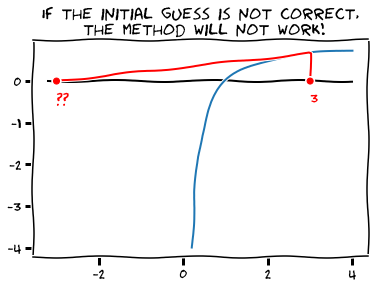
\includegraphics[width=0.55\linewidth]{images/badNewton.png}
\caption{Initial guess must carefully be chosen in Newton-Raphson}
\label{figure:NewtonRaphsonChoice}
\end{figure}
\end{example}

\begin{example}\label{example:NewtonRaphsonloop}
Consider now $f(x) = \sign(x)\sqrt{\lvert x \rvert}$ over $\field{R}$, with root at $x=0$.  The Newton-Raphson method fails miserably with this function: for any $x_0 \neq 0$
\begin{align*}
x_1 = x_0 - \frac{f(x_0)}{f'(x_0)} = x_0 - \frac{\sign(x_0)\lvert x_0 \rvert^{1/2}}{\tfrac{1}{2}\lvert x_0 \rvert^{-1/2}} = -x_0.
\end{align*}
This sequence turns into a loop: $x_{2n}=x_0$, $x_{2n+1}=-x_0$ for all $n\in \field{N}$ (see Figure \ref{figure:NewtonRaphsonloop}).
\begin{figure}[ht!]
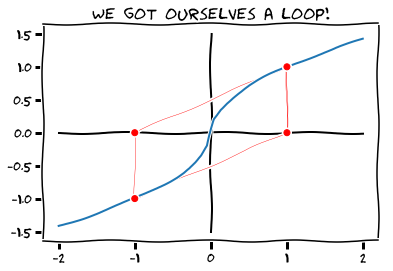
\includegraphics[width=0.55\linewidth]{images/loop.png}
\caption{Newton-Raphson fails for some functions}
\label{figure:NewtonRaphsonloop}
\end{figure}
\end{example}

\subsection{Efficiency of Newton-Raphson's Method}
To study the error in a Newton-Raphson iteration $\{ x_n \}_{n \in \field{N}}$ that converges to a root $x^\star$ of the function $f$, we observe that
\begin{align}
x_{n+1} - x^\star &= x_n - x^\star - \frac{f(x_n)}{f'(x_n)} \nonumber \\
&= (x_n - x^\star) \bigg( 1 - \frac{f(x_n)-\overbrace{f(x^\star)}^0}{(x_n-x^\star)f'(x_n)} \bigg) \nonumber \\
&= (x_n - x^\star) \bigg( 1 - \frac{1}{f'(x_n)} \frac{f(x_n) - f(x^\star)}{x_n - x^\star} \bigg) \label{eq:NRestimateStandBy}
\end{align}
Recall at this point the definition of \emph{divided differences} for any $n$--times differentiable function $g\colon \field{R} \to \field{R}$, and a family of values $t_0 \leq t_1 \leq \dotsb \leq t_n$:\index{Divided differences}
\begin{align*}
\Delta g[t_0,t_1] &= \frac{g(t_1)-g(t_0)}{t_1-t_0} \qquad\text{ (if }t_0 \neq t_1)\\
\Delta g[t_0,t_0] &= g'(t_0) \\
\Delta g[t_0,t_1,\dotsc,t_n] &= \frac{\Delta g[t_1, t_2, \dotsc, t_n] - \Delta g[t_0, t_1, \dotsc, t_{n-1}]}{t_n-t_0} \quad\text{(if }t_0 \neq t_n)\\
\Delta g[\underbrace{t_0, \dotsc, t_0}_{n+1 \text{ times}}] &= \frac{1}{n!} g^{(n)}(t_0) \qquad \text{(Why? \textbf{Hint:} Taylor's Polynomial)}
\end{align*}
We can then rewrite \eqref{eq:NRestimateStandBy} in terms of divided differences as follows:
\begin{align*}
x_{n+1} - x^\star &= (x_n - x^\star) \bigg( 1 - \frac{\Delta f[x_n, x^\star]}{\Delta f[x_n, x_n]}  \bigg) \\
&= (x_n - x^\star) \frac{ \Delta f[x_n, x_n] - \Delta f[x_n, x^\star] }{\Delta f [x_n,x_n]} \\
&= (x_n - x^\star) \frac{ \Delta f[x_n, x_n] - \Delta f[x_n, x^\star] }{x_n - x^\star} \frac{ x_n - x^\star }{\Delta f [x_n,x_n]} \\
& =(x_n - x^\star)^2 \frac{\Delta f[x_n, x_n, x^\star]}{\Delta f[x_n, x_n]}
\end{align*}
Therefore, 
\begin{equation*}
\lim_n \frac{x_{n+1}-x^\star}{(x_n - x^\star)^2} = \lim_n \frac{\Delta f[x_n, x_n, x^\star]}{\Delta f[x_n, x_n]} 
= \frac{f''(x^\star)}{2f'(x^\star)}.
\end{equation*}
If $f''(x^\star) \neq 0$, the Newton-Raphson's iteration exhibits quadratic convergence.\footnote{See Appendix \ref{appendix:convergence}}

\begin{remark} 
We have just proven that, if a Newton-Raphson iteration for a function $f$ gives a convergent sequence, the convergence is quadratic.  But, how can we guarantee convergence to a root of $f$?  The key is in \emph{how far can we start the sequence} given the structure of the graph of $f$.
\end{remark}

\begin{theorem}[Local Convergence for the Newton-Raphson Method]\label{theorem:LCNR}\index{Newton-Raphson!Local convergence for}
Let $x^\star$ be a simple root of the equation $f(x)=0$, and there exists $\varepsilon > 0$ so that 
\begin{itemize}
	\item $f$ is twice continuously differentiable in the interval $(x^\star-\varepsilon, x^\star + \varepsilon)$, and
	\item there are no critical points of $f$ on that interval.
\end{itemize}  
Set
\begin{equation*}
M(\varepsilon) = \max \bigg\{ \bigg\lvert \frac{f''(s)}{2f'(t)} \bigg\rvert : x^\star -\varepsilon < s,t < x^\star + \varepsilon \bigg\}.
\end{equation*}
If $\varepsilon$ is small enough so that $\varepsilon M(\varepsilon) < 1$, then 
\marginnote{I have seen this Theorem in \cite{gautschi2011numerical} with the condition $2 \varepsilon M(\varepsilon) < 1$ instead, but I could not see why that 2 was necessary.  What am I missing?}
\begin{enumerate}
	\item \label{thm:LCNR1} There are no other roots of $f$ in $(x^\star -\varepsilon, x^\star+\varepsilon)$.
	\item \label{thm:LCNR2} Any Newton-Raphson iteration starting at an initial guess $x_0 \neq x^\star$ in that interval will converge (quadratically) to $x^\star$
\end{enumerate} 
\end{theorem}
\begin{proof}
Start with Taylor's Theorem for $f$ around $x^\star$.  Given $x\neq x^\star$ satisfying $\abs{x-x^\star} < \varepsilon$, there exists $\xi$ between $x$ and $x^\star$ so that
\begin{align*}
f(x) &= f(x^\star) + (x-x^\star) f'(x^\star) + \tfrac{1}{2}(x-x^\star)^2 f''(\xi) \\
&= (x-x^\star)f'(x^\star) \bigg( 1 + (x-x^\star) \frac{f''(\xi)}{2f'(x^\star)} \bigg)
\end{align*}
Note that the three factors on the last expression are never zero:
\begin{align*}
x-x^\star &\neq 0 &&\text{(since }x \neq x^\star\text{ by hypothesis)} \\
f'(x^\star) &\neq 0 &&\text{(no critical points by hypothesis)} \\
\bigg\lvert (x-x^\star) \frac{f''(\xi)}{2f'(x^\star)} \bigg\rvert &\leq \varepsilon M(\varepsilon) < 1 &&\text{(by hypothesis on }M(\varepsilon))
\end{align*}
This proves \ref{thm:LCNR1}.

We want to prove now that all terms of a Newton-Raphson iteration stay in the interval $(x^\star - \varepsilon, x^\star + \varepsilon)$. We do that by induction:
\begin{itemize}
	\item $\abs{x_0 - x^\star}<\varepsilon$ by hypothesis.
	\item Assume $\abs{x_n-x^\star} < \varepsilon$.  In that case,
	\begin{equation*}
	\big\lvert x_{n+1} - x^\star \big\rvert = \big\lvert x_n - x^\star \big\rvert^2 \bigg\lvert \frac{\Delta f[x_n, x_n, x^\star]}{\Delta f[x_n, x_n]} \bigg\rvert
	\end{equation*}	
	but $\Delta f [x_n, x_n] = f'(x_n)$, and there exist $\xi_n$ between $x_n$ and $x^\star$ so that $\Delta f[x_n,x_n,x^\star] = \tfrac{1}{2}f''(\xi_n)$; therefore,
	\begin{equation*}
	\big\lvert x_{n+1} - x^\star \big\rvert = \big\lvert x_n - x^\star \big\rvert^2 \bigg\lvert \frac{f''(\xi)}{2f'(x_n)} \bigg\rvert \leq \varepsilon^2 M(\varepsilon) = \varepsilon \cdot \varepsilon M(\varepsilon) < \varepsilon.
	\end{equation*}
\end{itemize}
The next step is to prove that there is convergence.  A similar computation to the previous gives
\begin{equation*}
\big\lvert x_n - x^\star \big\rvert \leq \varepsilon M(\varepsilon) \big\lvert x_{n-1} - x^\star \big\rvert \leq \big( \varepsilon M(\varepsilon) \big)^n \big\lvert x_0 - x^\star \big\rvert.
\end{equation*}
Since $\varepsilon M(\varepsilon) < 1$, $\lim_n \big( \varepsilon M(\varepsilon) \big)^n = 0$, and $\{ x_n \}_{n \in \field{N}}$ converges to $x^\star$.
\end{proof}

\subsection{Extension to higher dimensions}

Let's proceed to extend this process to functions $\boldsymbol{g} \colon \field{R}^d \to \field{R}^d$ as follows.
\begin{itemize}
	\item Any function $\boldsymbol{g} \colon \field{R}^d \to \field{R}^d$ can be described in the form $\boldsymbol{g}(\x) = \big[ g_1(\x), g_2(\x), \dotsc, g_d(\x) \big]$ for $d$ real-valued functions $g_k\colon \field{R}^d \to \field{R}$ ($1\leq k \leq d$).
	\item For such a function $\boldsymbol{g}$, we may express its gradient as a $d\times d$ matrix in the form
	\begin{equation*}
	\gradient{\boldsymbol{g}} = \begin{bmatrix}
	\frac{\partial g_1}{\partial x_1} & \frac{\partial g_1}{\partial x_2} & \dotsb & \frac{\partial g_1}{\partial x_d} \\ \\
	\frac{\partial g_2}{\partial x_1} & \frac{\partial g_2}{\partial x_2} & \dotsb & \frac{\partial g_2}{\partial x_d} \\ \\
	\vdots & \vdots & \ddots & \vdots \\ \\
	\frac{\partial g_d}{\partial x_1} & \frac{\partial g_d}{\partial x_2} & \dotsb & \frac{\partial g_d}{\partial x_d} \\
	\end{bmatrix}
	\end{equation*}
\end{itemize}
Start with a guess for the solution, $\x_0$, and on the $n$--th step of the algorithm compute the $(n+1)$--th term of the sequence by
\begin{equation}\label{equation:NewtonMethod}
\x_{n+1} = \x_n - \big[ \gradient{\boldsymbol{g}}(\x_n) \big]^{-1} \boldsymbol{g}(\x_n),
\end{equation}
where $\big[ \gradient{\boldsymbol{g}}(\x_n) \big]^{-1}$ represents the inverse matrix of the gradient at $\x_n$.  This is equivalent to selecting in the tangent hyperplane to the graph of $\boldsymbol{g}$ at $\boldsymbol{g}(\x_n)$, the one line in the direction with the most rapid increase/decrease.  The computation of $\x_{n+1}$ is therefore the intersection of that line with the hyperplane $x_d=0$.  We refer to $\big[ \gradient{\boldsymbol{g}}(\x_n) \big]^{-1} \boldsymbol{g}(\x_n)$ as the \emph{Newton-Raphson direction} for $\boldsymbol{g}$ at $\x_n$.
\index{Newton-Raphson!direction}
\index{Newton-Raphson!method}
\index{Newton-Raphson!iteration}
\index{Newton-Raphson!Recursive formula}

\begin{example}\label{example:preNewton4poly4}
Consider the function $\boldsymbol{g}\colon \field{R}^2 \to \field{R}^2$ given by
\begin{equation*}
\boldsymbol{g}(x,y,z) = \big[ x^3-y, y^3-x \big]
\end{equation*}
Its gradient at each $(x,y)$ is given by
\begin{equation*}
\gradient{\boldsymbol{g}}(x,y) = \begin{bmatrix} 3x^2 & -1 \\ -1 & 3y^2 \end{bmatrix}
\end{equation*}
Note the determinant of this matrix is $\det \gradient{\boldsymbol{g}}(x,y) = 9x^2y^2-1 = (3xy-1)(3xy+1)$.  For any point $(x,y)$ that does not make this expression zero, this is an invertible matrix with 
\begin{equation*}
\big[ \gradient{\boldsymbol{g}}(x,y)\big]^{-1} = \frac{1}{9x^2y^2-1}\begin{bmatrix} 3y^2 & 1 \\ 1 & 3x^2 \end{bmatrix}
\end{equation*}
For an initial guess $(x_0, y_0)$, the sequence computed by this method is then given by
\begin{align*}
\begin{bmatrix} x_{n+1} \\ y_{n+1} \end{bmatrix} &= \begin{bmatrix} x_n \\ y_n \end{bmatrix} -\frac{1}{9 x_n^2 y_n^2-1}\begin{bmatrix} 3y_n^2 & 1 \\ 1 & 3x_n^2 \end{bmatrix} \begin{bmatrix} x_n^3-y_n \\ y_n^3-x_n \end{bmatrix} \\
% &= \begin{bmatrix}
% x_n - \frac{3x_n^3 y_n^2-2 y_n^3-x_n}{9x_n^2  y_n^2-1} \\  y_n - \frac{3x_n^2 y_n^3+-2x_n^3- y_n}{9x_n^2 y_n^2-1}
% \end{bmatrix}
\end{align*}
Let's run this process with three different initial guesses:
\begin{enumerate}
	\item Starting at $(x_0, y_0) = (-1.0,1.0)$, the sequence converges to $(0,0)$.  %See Table \ref{table:00}.
	\begin{center}
	% \begin{table}[ht!]
	\begin{tabular}{|c|c|c|} \hline 
	$n$ & $x_n$ & $y_n$ \\ \hline \hline 
	$0$ & $-1.00000000$ & $1.00000000$ \\ \hline 
	$1$ & $-0.50000000$ & $0.50000000$ \\ \hline 
	$2$ & $-0.14285714$ & $0.14285714$ \\ \hline 
	$3$ & $-0.00549451$ & $0.00549451$ \\ \hline 
	$4$ & $-0.00000033$ & $0.00000033$ \\ \hline 
	$5$ & $-0.00000000$ & $0.00000000$ \\ \hline 
	$6$ & $-0.00000000$ & $0.00000000$ \\ \hline 
	\end{tabular}
	% \caption{Newton Method: Convergence to $(0,0)$ with 8-digit accuracy in 5 steps}
	% \label{table:N00}
	% \end{table}
	\end{center}
	\item Starting at $(x_0,y_0) = (3.5, 2.1)$, the sequence converges to $(1,1)$.  %See Table \ref{table:11}.
	\begin{center}
	% \begin{table}[ht!]
	\begin{tabular}{|c|c|c|} \hline 
	$n$ & $x_n$ & $y_n$ \\ \hline \hline 
	$0$ & $3.50000000$ & $2.10000000$ \\ \hline 
	$1$ & $2.37631607$ & $1.57961573$ \\ \hline 
	$2$ & $1.65945969$ & $1.27476534$ \\ \hline 
	$3$ & $1.23996276$ & $1.10419072$ \\ \hline 
	$4$ & $1.04837462$ & $1.02274752$ \\ \hline 
	$5$ & $1.00260153$ & $1.00133122$ \\ \hline 
	$6$ & $1.00000824$ & $1.00000451$ \\ \hline 
	$7$ & $1.00000000$ & $1.00000000$ \\ \hline 
	$8$ & $1.00000000$ & $1.00000000$ \\ \hline 
	\end{tabular}
	% \caption{Newton Method: Convergence to $(1,1)$ with 8-digit accuracy in 7 steps}
	% \label{table:N11}
	% \end{table}
	\end{center}
	\item Starting at $(x_0, y_0) = (-13.5, -7.3)$, the sequence converges to $(-1,-1)$.  %See Table \ref{table:-1-1}.
	\begin{center}
	% \begin{table}[ht!]
	\begin{tabular}{|c|c|c|} \hline 
	$n$ & $x_n$ & $y_n$ \\ \hline \hline 
	$0$ & $-13.50000000$ & $-7.30000000$ \\ \hline 
	$1$ & $-9.00900415$ & $-4.92301873$ \\ \hline 
	$2$ & $-6.01982204$ & $-3.36480659$ \\ \hline 
	$3$ & $-4.03494126$ & $-2.36199873$ \\ \hline 
	$4$ & $-2.72553474$ & $-1.73750959$ \\ \hline 
	$5$ & $-1.87830623$ & $-1.36573112$ \\ \hline 
	$6$ & $-1.36121191$ & $-1.15374930$ \\ \hline 
	\end{tabular}~\begin{tabular}{|c|c|c|} \hline
	$n$ & $x_n$ & $y_n$ \\ \hline \hline 
	$7$ & $-1.09518303$ & $-1.04341362$ \\ \hline 
	$8$ & $-1.00932090$ & $-1.00463507$ \\ \hline 
	$9$ & $-1.00010404$ & $-1.00005571$ \\ \hline 
	$10$ & $-1.00000001$ & $-1.00000001$ \\ \hline 
	$11$ & $-1.00000000$ & $-1.00000000$ \\ \hline 
	$12$ & $-1.00000000$ & $-1.00000000$ \\ \hline 
	$13$ & $-1.00000000$ & $-1.00000000$ \\ \hline 
	\end{tabular}
	% \caption{Newton Method: Convergence to $(-1,-1)$ with 8-digit accuracy in 11 steps}
	% \label{table:N-1-1}
	% \end{table}
	\end{center}
\end{enumerate}
\end{example}

\subsection{Optimization via Newton's Method}
We can readily see how this process aids in the computation of critical points of twice continuously differentiable real-valued function $f\colon \field{R}^d \to \field{R}$:
\begin{enumerate}
	\item Set $\boldsymbol{g}(\x) = \gradient{f}(\x) = \big[ \frac{\partial f}{\partial x_1}, \dotsc, \frac{\partial f}{\partial x_d} \big]$
	\item It is then $\gradient{\boldsymbol{g}}(\x) = \Hess{f}(\x)$
	\item Perform a Newton method (with initial guess $\x_0$) on $\boldsymbol{g}=\gradient{f}$ to obtain the recurrence formula
	\begin{equation}\label{equation:Newton4Crit}
	\x_{n+1} = \x_n - \big[ \Hess{f}(\x_n) \big]^{-1} \cdot \gradient{f}(\x_n)
	\end{equation}
\end{enumerate}

\begin{example}\label{example:NewtonPoly4}
Consider the polynomial $p_4(x,y) = x^4-4xy+y^4$. Notice $\gradient{p_4}(x,y) = \big[ x^3-y, y^3-x \big]$---this is function $\boldsymbol{g}$ in Example \ref{example:preNewton4poly4}.  The critical points we found were $(0,0)$, $(-1,-1)$ and $(1,1)$.  See Figure \ref{figure:NewtonConvergence}.
\end{example}
\begin{example}
A similar process for the Rosenbrock function\index{Function!Rosenbrock} 
\begin{equation*}
\mathcal{R}_{1,1}(x,y) = (1-x)^2 + (y-x^2)^2
\end{equation*}
gives the following recurrence formula:
\begin{align*}
\begin{bmatrix} x_{n+1} \\ y_{n+1} \end{bmatrix} &=
\begin{bmatrix} x_{n} \\ y_{n} \end{bmatrix} - \big[ \Hess{\mathcal{R}_{1,1}}(x_n,y_n) \big]^{-1} \cdot \gradient{\mathcal{R}_{1,1}}(x_n, y_n) \\
% &= \begin{bmatrix} x_{n} \\ y_{n} \end{bmatrix} - \tfrac{2}{2x^2-2y+1} \begin{bmatrix}
% 1/2 & x_n \\ x_n & 6x_n^2-2y_n+1
% \end{bmatrix} \begin{bmatrix}
% 2x_n^3-2x_n y_n +x_n -1 \\ y_n -x_n^2
% \end{bmatrix} \\
&= \frac{1}{2x_n^2-2y_n+1} \begin{bmatrix}
2x_n^3-2x_n y_n+1 \\ x_n(2x_n^3-2x_n y_n-x_n+2)
\end{bmatrix}
\end{align*}
For instance, starting with the initial guess $(x_0, y_0) = (-2,2)$, the sequence converges to the critical point $(1,1)$.  See Figure \ref{figure:NewtonConvergence}.
\end{example}
\begin{figure}[ht!]
\begin{tabular}{cc}
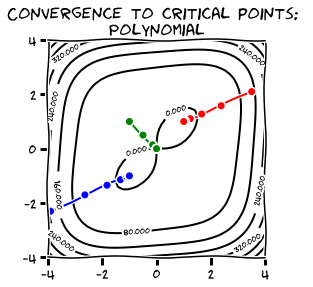
\includegraphics[width=0.45\linewidth]{images/convergenceNewton.png} &
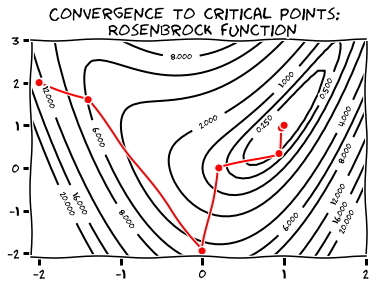
\includegraphics[width=0.55\linewidth]{images/convergenceNewtonRosenbrock.png} 
\end{tabular}
\caption{Newton-Raphson method}
\label{figure:NewtonConvergence}
\end{figure}

\begin{remark}
The Newton-Raphson's method to solve $\boldsymbol{g}=\boldsymbol{0}$, as given by the recurrence formula in equation \eqref{equation:NewtonMethod} in page \pageref{equation:NewtonMethod}, is very convenient to provide explicit descriptions of the different iterations.  However, it is hardly suitable for practical purposes, due to the computational issues involving matrix inversion.\index{Matrix!inversion}\index{Matrix!inverse}

To avoid dealing with matrix inversion, we consider the following equivalent formula:
\begin{equation}
\gradient{\boldsymbol{g}}(\x_n) \cdot \big( \x_{n+1} - \x_n \big) = -\boldsymbol{g}(\x_n)
\end{equation}
This is a simple system of linear equations, a much more reliable process, prone to less numerical error.

The equivalent recurrence formula to search for critical points of a twice continuously differentiable real-valued function $f \colon \field{R}^d \to \field{R}$ is thus
\begin{equation}
\Hess{f}(\x_n) \cdot (\x_{n+1}-\x_n) = -\gradient{f}(\x_n).
\end{equation}
\end{remark}

\begin{example}
The equivalent recurrence formula to the one we obtained in example \ref{example:preNewton4poly4} is as follows:
\begin{equation*}
\begin{bmatrix} 3x_n^2 & -1 \\ -1 & 3y_n^2 \end{bmatrix} \begin{bmatrix} x_{n+1}-x_n \\ y_{n+1}-y_n \end{bmatrix} = \begin{bmatrix} x_n^3 - y_n \\ y_n^3 - x_n \end{bmatrix}
\end{equation*}
All we need to do is, at each step $n$, solve for $X$ and $Y$ the system of linear equations
\begin{equation*}
\begin{cases}
3x_n^2 (X-x_n) - (Y-y_n)  = x_n^3 - y_n \\
-(X-x_n) + 3y_n^2 (Y-y_n) = y_n^2 - x_n
\end{cases}
\end{equation*}
or equivalently,
\begin{equation*}
\begin{cases}
3x_n^2 X - Y = 4x_n^3 - 2y_n \\
-X + 3y_n^2 Y = 4y_n^2 - 2x_n
\end{cases}
\end{equation*}
\end{example}

\separator

There are some theoretical results that aid in the search for a \emph{good} initial guess in case of multivariate functions.  The following states a simple set of conditions on $f$ and $\x_0$ to guarantee \emph{quadratic convergence} of the corresponding sequences $\{ \x_n \}_{n \in \field{N}}$ to a critical point $\xstar$.

\begin{theorem}[Quadratic Convergence Theorem]\label{theorem:QuadraticConvergence}\index{Theorem!Quadratic Convergence}
Suppose $f\colon \field{R}^d \to \field{R}$ is a twice continuously differentiable real-valued function, and $\xstar$ is a critical point of $f$. Let $\mathcal{N}(\x) = \x - \big[ \Hess{f}(\x) \big]^{-1} \cdot \gradient{f}(\x)$. If there exists 
\begin{enumerate}
	\item $h>0$ so that\footnote{Recall the \emph{norm} of a matrix $M$, defined by $\norm{M} = \max\{ \norm{M\cdot \x} : \norm{\x}=1 \}$.} $\big\lVert \big[ \Hess{f}(\xstar)\big]^{-1} \big\rVert \leq \tfrac{1}{h}$,
	\item $\beta>0$, $L>0$ for which $\norm{\Hess{f}(\x) - \Hess{f}(\xstar)} \leq L \norm{ \x - \xstar }$ provided $\norm{ \x - \xstar }\leq \beta$.
\end{enumerate}
In that case, for all $\x \in \field{R}^d$ satisfying $\norm{ \x - \xstar }\leq \min \{\beta, \tfrac{2h}{3L} \}$,
\begin{equation*}
\frac{\norm{ \mathcal{N}(\x) - \xstar }}{\norm{\x - \xstar}^2} \leq \frac{3L}{2h}
\end{equation*}
\end{theorem}